\documentclass[a4paper,11pt]{article}
%%%%%%%%%%%%% image %%%%%%%%%%%%%%%%%
\usepackage{graphicx}
\usepackage[utf8]{inputenc}
\usepackage[english]{babel}
\usepackage{lscape}
\usepackage{rotating}
%%%%%%%%%%%%%%%%%%%%%%%%%%%%%%%%%%%%

%\usepackage{hyperref} % to draw square on reference number
\usepackage{url}

%%%%%%%%%%%%%%%% cite %%%%%%%%%%%%%%
\usepackage[numbers]{natbib}
%\citestyle{nature}
\usepackage{usebib}
\newbibfield{editor}
\newbibfield{author}
\newbibfield{publisher}
\bibinput{proposal}
%%%%%%%%%%%%%%%%%%%%%%%%%%%%%%%%%%%%

%%%%%%%%%%%%%%%%%%%%%%%highlight%%%%
\usepackage{xcolor}
\usepackage{color, soul}
\sethlcolor{yellow}

\usepackage{soul}
\usepackage{color}
\soulregister\cite7
\DeclareRobustCommand{\hlyellow}[1]{{\sethlcolor{white}\hl{#1}}}
\DeclareRobustCommand{\hlred}[1]{{\sethlcolor{red}\hl{#1}}}

\pagenumbering{roman}

%%%%%%%%%%%% margins %%%%%%%%%%%%%%%%
 \addtolength{\oddsidemargin}{-.875in}
 \addtolength{\evensidemargin}{-.875in}
 \addtolength{\textwidth}{1.95in}              %1.75in
 \addtolength{\textheight}{1.75in} 
 \addtolength{\topmargin}{-.875in}
%%%%%%%%%%%%%%%%%%%%%%%%%%%%%%%%%%%%%

%%%%%%%%space between lines%%%%%%%%%
\usepackage{setspace}
%\doublespacing
%\onehalfspacing
%\singlespacing
%\linespread{1.1}
%%%%%%%%%%%%%%%%%%%%%%%%%%%%%%%%%%%%


\begin{document}
\begin{titlepage}
\begin{center}
%fig0
\begin{figure} [htp] 

\includegraphics[width=1\columnwidth]{pic/USQ.png}
\label{fig:fig0}
\end{figure} 
   
    {\bfseries\Large
        \begin{center}
        \huge{Incorporating Security into Healthcare Applications of WSNs}
        \end{center}         
   %     \newline
        \vskip2cm
       \LARGE{PhD Research Proposal}\\
       
        \vskip.5cm
       \normalsize{ Faculty of Health, Engineering and Sciences \\
        School of Agricultural, Computational and Environmental Sciences}\\
        
        \vskip2cm
        \normalsize{Candidate: Mishall Al-Zubaidie\\
                    Student ID: 0061070801}\\   
                   
        \vskip1cm
        \normalsize{Supervisors:\\
                    Dr. Zhongwei Zhang\\
                    Dr. Ji Zhang\\
                    \vskip2cm 
                    March 2017}                           
    }    
    %\vfill    
    \end{center}
\end{titlepage}

\onehalfspacing
\tableofcontents


\newpage
\doublespacing

\begin{abstract}
Recent years have witnessed the development of different embedded computing systems that incorporate processing, storage, wireless communications, remote administration and sensor devices. The potential of applying wireless sensor network (WSN) and electronic healthcare record (EHR) in the healthcare (HC) industry are tremendous and boundless, while user acceptance would grow exponentially, subject to the fact that users have great confidence in the system. However, the application of WSN in healthcare services may be vulnerable to many attacks and data collected/stored on the healthcare system is required to be securely communicated among users. The security issue of healthcare data must be addressed with great caution and accessibility. Compared with traditional healthcare systems which use paper record systems, adopting and moving on to EHR is a general trend in healthcare industries since EHR systems are considered capable of providing more efficiency, are less error prone and have higher availability. The EHR system security and privacy are related to the issues of confidentiality of protected health information (PHI), the integrity of EHRs and authentication of users. While EHR data are collecting, communicating among different users' access, along with the sharing of the patient health data.\\

On the basis of these advanced technologies, and the assumption of providing better quality and cost effective service. In this study, we will develop and build up a prototypical EHR-based healthcare system. The proposed healthcare system will be implemented by: (1) using WSN, a technique to automatically collect patient EHR; (2) taking advantage of EHR repository; and (3) relying on an extensible access control markup language (XACML) to secure communicate EHR among healthcare providers and users. In this proposal, we propose using elliptic curve cryptography (ECC) and elliptic curve digital signature algorithm (ECDSA) algorithms because these algorithms provide high performance and security in WSN compared other asymmetric and symmetric algorithms. But because of the increasing attacks on WSN, some protocols are needed to improve security and efficiency against various attacks. Also, a critical component of the proposed healthcare system is a patient information repository or patient's healthcare database server.  Patients' database in the server needs protection and data management. We propose the use of XACML to manage and access control users (patients and healthcare members) to the database. Such a prototype of the WSN based system would provide better healthcare services with security to various healthcare professionals, including patients. 
\end{abstract}
\newpage


%\setcounter{page}{3}
\pagenumbering{arabic}
\section{Introduction}
%\setlength{\baselineskip}{1.6\baselineskip}
Wireless sensor network (WSN) technology is widely used in recent years in several applications such as healthcare (HC), military, government security policy, environment, office/home automation, education and transportation \cite{pr9,pr3,pr5}. This type of networks provides comfort and safety to humans by monitoring a specific area without human intervention or the presence \cite{pr1}. An important application that brought the attention of many researchers to sensor networks is healthcare because it is great importance in our lives to reduce the effects of diseases on the health of patients. Providing better healthcare quality of lower cost will be the key aim of all health industry over the next decades.

\subsection{Healthcare and Information and Communications Technology}
Many countries have reprioritized the healthcare industry \hlyellow{after} the defense and military in terms of budget and strategy \cite{pr44}; it is becoming increasingly evident that advanced Information and Communications Technology (ICT) holds the key to the success of providing better healthcare quality at \hlyellow{lower} cost. Healthcare services have become so diversified \hlyellow{and demanding} that providers of ICT such as WSN and electronic health record (EHR) systems have to be used in order to deliver efficient but affordable services to the broader healthcare users and communities. These WSNs promise to significantly enhance the care quality over a wide range of clients populations.  

\subsection{WSN Applications in Healthcare}
Healthcare is one of the important and sensitive applications that offer quality-of-care for patients. It has been designed to improve the health status of patients and thus reduce the harmful effects of diseases. Moreover, there are many organizations that provide standards for healthcare applications such as Health Level Seven (HL7), Health Insurance Portability and Accountability Act (HIPAA). These standards are very important \hlyellow{when creating a healthcare} application. These applications have become more efficient with the use of WSN; the applications of such kind are known as healthcare wireless sensor networks (HWSN).  \cite{pr1}. By using HWSN, physicians can get information about patients on an ongoing basis, whether at home or in hospital because this information leads to the correct diagnosis and thus the improvement of the patient's condition. Where there are a lot of diseases that require constant monitoring and precise care. For example, HWSN is the best method used by doctors to get patient information, as this technology provides patients with comfort and more care at less cost \cite{pr1}. These applications monitor patient activities without interruption, which leads to improved health condition \cite{pr11}. The architecture of HWSN is shown in Figure \ref{fig:archwsn2}. This architecture consists of three layers are sensors, communication equipment and back-end network. This proposal will focus on three aspects of HWSN data:
\begin{itemize}
\item \textbf{Healthcare data collection}\\
In the first aspect, sensors collect data about the patient continuously and send it to the server. The data collected properly helps doctors diagnose the diseases accurately. Also, patients' data collection needs protection from intrusion.

\item \textbf{\hlyellow{Healthcare data structure}}\\
The second aspect is the data storage in the form of tables of a server's database. The data structure for EHR repository should be able to facilitate the sharing of a patient's health information among the healthcare professionals. 

\item \textbf{Healthcare data access and privacy}\\
The third aspect is to determine who has the right of users (doctor, nurse, general practitioner, pharmacist and government officer) in the access to these tables. All these stages require security and privacy mechanisms to protect the EHR.
\end{itemize}

%fig1
\begin{figure}[t]
	\centering
		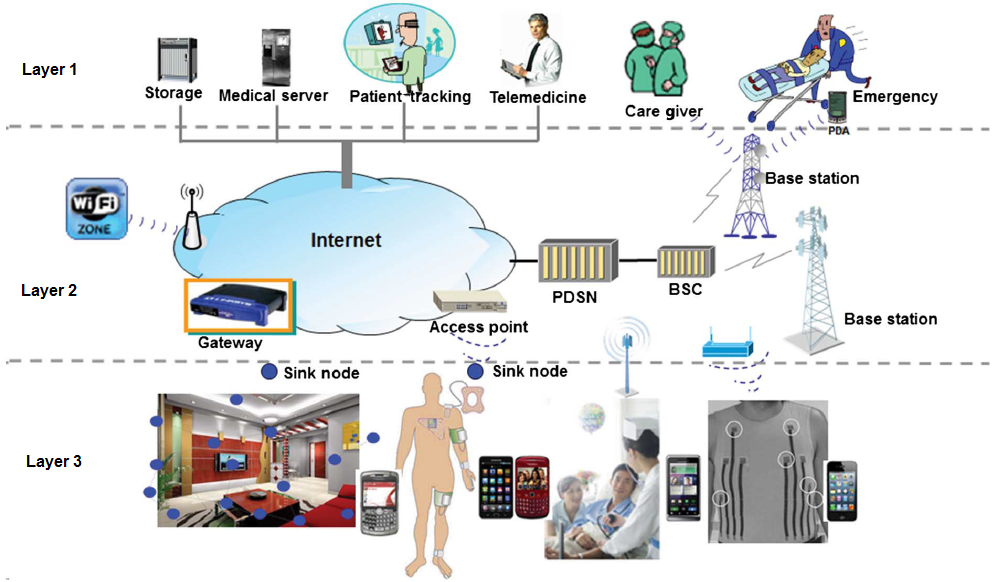
\includegraphics[width=15cm,height=8cm]{pic/archwsn2.png}
	\caption{Architecture of healthcare based WSN \cite{pr6}}
	\label{fig:archwsn2}
\end{figure}

\subsection{Security and Privacy in the Healthcare Applications}
In this section, we will discuss the risks and security weakness to healthcare applications of WSN. There are several attacks that threaten the WSN used to collecting patient's healthcare data and to the security of the EHR repository. These attacks have been classified into passive and active attacks \cite{pr8}. In all types of passive attacks, an adversary eavesdrops the transmitted packets between network nodes and server. Also, the attacker analyzes these packets to reveal information without change (i.e. trying to break the confidentiality) such as eavesdropping and traffic analysis attacks. \hlyellow{The active type} of attack is very harmful to the networks of healthcare applications. An attacker alters data packets and sends them back to their destination such as masquerading, reply, modification and denial of service attacks \cite{pr19}. Also, there is \hlyellow{another classification} of attacks on healthcare applications is internal and external attacks. In the internal attacks, the attacker is a member of the network. This type of attacks is more dangerous than external attacks because the internal attacker has the authority to send and receive messages, \hlyellow{which means} an attack from the inside is easier. Figure \ref {fig:hackeav} describes the attacks on the WSNs which are used to infiltrate data collected/stored.

%fig2
\begin{figure}[t]
	\centering
		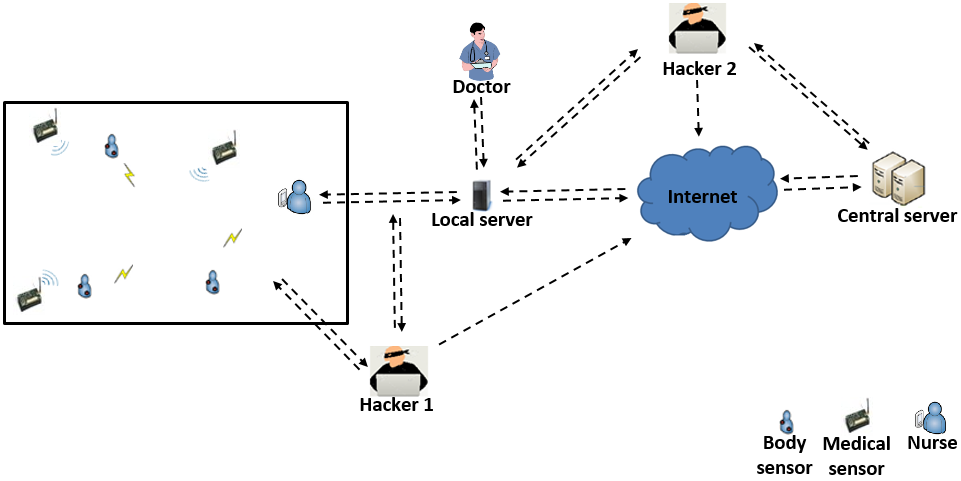
\includegraphics[width=15cm,height=8cm]{pic/hackeav.png}
	\caption{An attack on information security (hacker 1) and device security (hacker 2)}
	\label{fig:hackeav}
\end{figure}

An attacker listens \hlyellow{to information} as it is transferred from the patients' sensors to the server or performs an attack on the server to penetrate the database to get the patients' information, as shown in Figure \ref{fig:hackeav}. When the attacker gets the message, he can \hlyellow{get information about} the physical location of the patient, ID, timestamps, source address, target address and the medical report sent by the sensors or directed by medical staff. Also, an attacker can get information from the database, such as the patient's name, age, address, type of disease, and the seriousness of the disease. This information allows the attacker to harm the patient in different ways \cite{pr1}. The patient information transmitted through the sensor networks requires complete privacy, especially if patient information through the network does not require the consent of the patient, such as moving data through an emergency case. Therefore, privacy and security issues are very important in healthcare applications. If these applications do not provide adequate security for the patient's information, these applications become useless and unusable because the disclosure of patients' information that may affect their health or even death.

Most of these attacks can be cancelled \hlyellow{when the security} requirements, in particular, confidentiality, authentication and integrity in \hlyellow{the network are addressed} properly and appropriately. To prevent attacks of HWSN applications should add the appropriate security services. \hlyellow{These services should protect} data from tampering, modification or eavesdropping. The security of the healthcare applications includes:

\begin{itemize} 
\item \textbf{Confidentiality} data encrypted through the encryption algorithm to prevent the attacker from seeing explicit data. When the attacker gets the encrypted data, the attacker will not benefit from this data because it is incomprehensible \cite{pr15}. 
\item \textbf{Authentication and Authorization} authentication service is used to authenticate legitimate users or data in the network to prevent anyone else. This means that if the data is a trusted source in the network it is accepted, but if an unknown source is ignored \cite{pr16}. While in the authorization service, each node in the network has specific sources that can access it. This security requirement is very important in preventing unauthorized persons' access to the sources, for example, providing various privileges among users (doctors, nurses, practitioners and pharmacists) in access to the sources \cite{pr11}. 
\item \textbf{Integrity} this service is used to ensure that the transmitted data that has not been tampered or edited by the adversary \cite{pr18}. 
\end{itemize} 

The following concerns closely related to patient's EHR: 
\begin{itemize} 
\item \textbf{Availability} there are some attacks try to disrupt network services, by sending a large number of messages to the server and thus the network destruction. Network services should be available upon request \cite{pr14}. 
\item \textbf{Anonymity} this service is to hide or distort the network data as it transfers from the sender to the receiver or vice versa. When using anonymity with the data, the attacker cannot distinguish this data to a specific patient \cite{pr22} \item \textbf{Scalability, Forward Secrecy and Backward Secrecy} environments of healthcare applications require expanding the size of the network continuously, but when a node leaves or joins the network, it does not have the right to access and decrypt the encrypted messages in future after leaving the network or previous messages before entering the network. 
\item \textbf{Freshness and Non-repudiation} the message should be recent to prevent a replay attack, as the sender cannot deny his message to detect the compromised nodes \cite{pr14,pr17}.
\end{itemize}

\subsection{\hlyellow{Significance of the Project}}
\hlyellow{The healthcare application has offered great benefits to the society through providing care for patients and improving their health. Collecting of patients' information and storing it in servers makes the transfer of information faster and more accurate among health centers. However, collecting of modified or inaccurate data (because of the attacks) and storing them on the server as well as access the unauthorized server's database cause significant harm to patients' health. Also, data exchange between different devices in the network requires data security management to deal with medical records in a flexible and accurate manner. The lack of protection of patients' information adversely affects the treatment of patients, which leads to harm, reduced dignity, stigma, discrimination, embarrassment or even death. Many research studies have shown that patients and professionals in hospitals or clinics have been interested in issues of information security (personal and health information) and protect the rights of patients from tampering. Therefore, the security and privacy of patients' information are a prerequisite and paramount importance to the creation of healthcare application which is a great concern in the society. The research described in this proposal has addressed the security and privacy significance as the following to provide a safe environment for the transfer and storage of medical records for patients.}
\begin{itemize}
\item \hlyellow{Protecting of the patients' data collected continuously by WSN to prevent data modification}.
\item \hlyellow {Data security management}
\item \hlyellow{Determining of the access authorized users (privacy) to the patients' database stored on servers}.  
\end{itemize}


\section{Research Objectives, Questions and Our Contributions}
In this section, we will list the objectives and problems for our research.  

\subsection{Research Objectives}
The following objectives are laid out to achieve in our project research.

\begin{itemize}
\item \textbf{Automate healthcare data collection using WSN} \\ 
Manually collecting healthcare data is expensive and error-prone. Using WSN to automatically collect and convert to electronic records can significantly improve quality and reduce the cost of the healthcare. In many environments where healthcare professionals such as nurses and doctors are in practical to monitor patients. WSN can be deployed to continuously monitor a patient's condition and gather data all the time.
\item \textbf{Efficient healthcare data management using EHR and XML}\\
Patient data transmitted between sensors (nodes and cluster head) and network devices (such as a nurse and a server device) need data management algorithms to maintain both performance and security at the same time. EHR including patient's confidential data and private information needs to be accessed by healthcare professionals, thus sharing such EHR without breaching a patient's privacy requires EHR management in an efficient and secure manner. XML technology has begun showing its superiority in the exchanging of complex data over different systems.
\item \textbf{Beef up healthcare privacy and security using XACML and XML signencryption}\\
When all patient information is stored on a server, that server becomes attractive to attackers. Therefore, the use of security mechanisms to determine access to the server is a very important issue. All protected health information (PHI) stored in the EHR repository should be been encrypted and XML signencryption technology would be applied to achieve maximum security. 
\end{itemize}


\subsection{Specific Research Questions}
In this section, we will describe some problems that might threaten the privacy and security of information in the proposed healthcare system. That is, we intend \hlyellow{to investigate} the following research problems to complete our study.
\begin{enumerate}
\item \emph{How WSNs can help collect a patient's healthcare data within an EHR system?
\item How \hlyellow{to transfer} healthcare data for WSN to the EHR repository securely?
\item How \hlyellow{to authorize} healthcare professionals \hlyellow{when accessing} the healthcare information from the EHR repository?
\item How to update the EHR information stored in the repository while maintaining privacy?}
\end{enumerate}

\subsection{\hlyellow{Our Contributions}}
\hlyellow{In this section, we will clarify our contributions in this research as follows:}
\begin{enumerate} 
\item \hlyellow{We will design a new way of collecting patients' data based on Quark hash algorithm to prevent attacks such as collision and preimage attacks.}

\item \hlyellow{We will develop a new communication algorithm (ECC/ECDSA) based on homomorphic properties, encryption of 1 scalar multiplication and using of XML technology to manage encrypted patients\rq data.} 

\item \hlyellow{We will develop a new way of access users for patients' database. First, we will merge ECDSA with anonymity in a single node. This means that our contribution is dependent on the signature parameters ($k, r, s$) and not on the signing of the other nodes. This scheme will provide a great security against the compromised nodes. Second, we will develop an application based on XACML, signencryption and anonymity to determine the access of users (professionals and patients) to medical records in the repository.}
\end{enumerate}


\section{\hlyellow{Literature Review}}
~~~In this section, we will present the literature review about the security of patient data in WSN and healthcare applications. We will focus on a study on the security and performance aspects (ECC/ECDSA) in HWSN and privacy and confidentiality in EHR.
\subsection{\hlyellow{Improvement of Service and Communication in WSN Security and Performance}}
The authors in \cite{p40} used a number of small bits to specify the number of allowed points in point multiplication. Similarly, \citeauthor{p25}(\citeyear{p25}) in \cite{p25} presented a method to generate $k$ depending on the generation of an integer $S$ periodically to reduce point additions. \hlyellow{Both previous schemes suffered from a lack of randomization due to the determination of random values in ephemeral $k$}. Also, the modified SHA-1 algorithm was proposed for use with a pre-shared secret key  \cite{p34}. It exchanged logic functions to pseudo-random function plus a secret key $k_s$ to reduce the cost of computation and communication in WSN. \hlyellow{This scheme improved the performance of the algorithm significantly, but this improvement was at the expense of security}. In addition, \citeauthor{p26}(\citeyear{p26}) in \cite{p26} discussed increasing the security level in ECDSA algorithm through using $F_{2^{233}}$ with SHA-224 and Montgomery algorithm. They explained that $F_{2^m}$ is faster than $F_p$ while $F_p$ is more secure. \hlyellow{According to several research that key 233 is hacked and vulnerable to attacks}. Furthermore, \citeauthor{p12}(\citeyear{p12}) in \cite{p12} removed the inversion process in ECDSA to reduce running time on Micaz sensor. They improved the performance of ECDSA but did not prove the security level. The \citeauthor{p8}(\citeyear{p8}) in \cite{p8} used a few keys (broadcast only session keys with periodic authentication in session key) to save resources and reduce the computation in ECDSA, but their scheme suffered from a storage problem in WSN. However, all these research papers suffered from collision and preimage attacks because these research papers had used SHA-1. \hlyellow{In our scheme, we will integrate the Quark algorithm with ECDSA to address both security and performance, the Quark algorithm has immunity to hash algorithm attacks and is suitable for source restricted devices (WSN).}\\
Encryption and signing algorithms were used for the collected data \cite{p11,p15}. Encryption algorithm EC-OU (Elliptic Curve Okamoto-Uchiyama) was used to maintain confidentiality and ECDSA algorithm to maintain integrity; both algorithms were used during homomorphic. \hlyellow{This approach needed large computations to complete the factoring issue so it suffered from delays because the complexity of the operations and the authors did not specify the key size and the type of field used}. Similarly, the improvement was proposed for signature verification in ECDSA through cooperating of adjacent nodes in the computation of intermediate results (with 1 scalar multiplication (SM)) on Micaz motes with the finite field ($F_{2^{163}}$) \cite{p46,p17}. \hlyellow{This scheme used several hops to transmit data to a destination that makes it vulnerable to attacks and SM's result was not protected}. Also, \citeauthor{pr35}(\citeyear{pr35}) in \cite{pr35} used the homomorphic with ECC and ElGamal on Micaz. They used the Comb method in the SM to prevent SPA attacks. \hlyellow{Their scheme required complex processes due to the use of the Elgamal algorithm as well as the use of the Comb method which is consumed for storage (precomputations of points)}. \hlyellow{We will adopt both schemes in \cite{p17, pr35} but with the use of one hop, prime field, protection of 1 SM's result and ECC/ECDSA to provide protection and performance in the collection and transmission of patients' data through our communication protocol}. According to our survey paper \cite{p93} and the best knowledge we have, authors used small keys through using ECC/ECDSA in WSN as well as the use of the consuming algorithms for sources such as ElGamal and binary field least security. These small keys make WSN vulnerable to attacks. Moreover, authors in \cite{p9,p87,pr24} proved the possibility of the use of RSA and ECC/ECDSA algorithms in several types of sensor nodes (Mica2dot, Mica2, Micaz and TelosB). They pointed out that the ECC/ECDSA algorithms provide better performance in terms of speed and storage than RSA.

\subsection{\hlyellow{Using Anonymity Property to Secure WSN and EHR}}
\citeauthor{pr22}(\citeyear{pr22}) in \cite{pr22} proposed the use of $k$-anonymity with the patient's database to allow the sharing of patient information distorted publicly. Also, \citeauthor{p78}(\citeyear{p78}) in \cite{p78} used an SHA-1 algorithm to generate ephemeral $k$ and to gain appropriate randomness to increase signature security as a countermeasure against side channel attacks. While \citeauthor{pr23}(\citeyear{pr23}) in \cite{pr23} incorporated anonymity property with ECDSA in vehicular ad hoc network applications. They used the node ID and the time the encrypted by the hash algorithm in the generation and signature verification. Furthermore, both authors in \cite{p78,p27} enhanced signature equation in ECDSA to hide access private key and to prevent DPA or CPA attacks. \hlyellow{The improvement of the signature equation has increased the complexity of computation processes and 
the lack of protection against side channel attacks}. \citeauthor{pr34}(\citeyear{pr34}) in \cite{pr34} suggested the use of ECC with AC through dividing network users to groups as well as the use of ring signature to prevent attackers from reaching the message source. \hlyellow{The problem in their scheme was that the computers sign the messages and sensors that verify the messages' signature in addition to the use of ring signature method that has consumed for energy}. Similarly, \citeauthor{pr33}(\citeyear{pr33}) in \cite{pr33} presented an authentication scheme of hop by hop depending on ECC and ElGamal algorithms with anonymity. In their scheme, the source node was used to choose a set of intermediate nodes to transfer the message to the destination node. \hlyellow{Their protocol was consumed for time and energy because the message is signed several times to reach the destination}. All of these schemes in this section suffered from side channel attacks and very expensive in WSNs. \hlyellow{In our research, we will adopt the scheme in \cite{pr22} to hide the patient's records in the server and not to share them in general. Also, we will adopt the scheme in [37] but with ECC/ECDSA, in addition, authentication will implement through using of ECDSA with anonymity in one node rather than several nodes.}

\subsection{\hlyellow{AC Mechanisms to Protect EHR's Repository}}
The authors in \cite{pr42} explained that XACML is a very important component in distributed systems, while authors in \cite{pr52} suggested the use of service-oriented architecture (SOA) with the EHR to provide shared data service and security features. They suggested the use of XML encryption to protect access to EHR data, \hlyellow{but did not state the encryption algorithm}. \citeauthor{pr56}(\citeyear{pr56}) in \cite{pr56} designed and carried out a prototype system dependent on the Web and focused on the participation of providers' access to patient data (EHR). They used the central database with several local databases \hlyellow{without attention to security issues}. This system was designed by JavaScript and HTML and databases were developed by MS-SQL. Also, \citeauthor{p19}(\citeyear{p19}) in \cite{p19} implemented ECC/ECDSA algorithm (Sliding window method) ($F_P$) with AC schemes, then compared their scheme with two different schemes (ECCM and TinyECC). \hlyellow{Their scheme was inappropriate for resources such as storage due to using of the slide window method}. Moreover, \citeauthor{pr47}(\citeyear{pr47}) in \cite{pr47} presented the openEHR project as an archetype model to be used for the construction of EHR systems. The authors have made a review of the specification of the architecture of this project. They focused on security issues, privacy and AC in the EHR. \hlyellow{Their archetype did not discuss the use of WSN, which is an important component in data collection}. Also, \citeauthor{pr25}(\citeyear{pr25}) in \cite{pr25} suggested the use of AC with the ECC in the WSN. The authors focused on the authentication of the new nodes. They pointed out that their scheme is able to prevent malicious nodes from joining the network through the use of node ID and bootstrapping time in addition to the establishment of a shared key between adjacent nodes. Similarly, \citeauthor{pr24}(\citeyear{pr24}) in \cite{pr24} proposed AC with ECC in the WSN. They have suggested the mutual authentication and key establishment on the ECC algorithm. They also used the freshness, forward and backward secrecy properties with session keys. \hlyellow{Complex processes (shared keys) were used in their scheme that were complicated the access professionals to health information for the patient}.\\
~~~Also, authors in \cite{pr46} designed an EHR system to protect the confidentiality of patient data. They focused on the emergency state in the protection of patient data through the use of a back-up mechanism (Shamir scheme) that allows the physician access to the patient's health information without access to confidential parameters. Moreover, authors in \cite{pr49, pr54} designed an EHR scheme dependent on many keys and pseudonym property to prevent the link patient definitions with health information. But these schemes \cite{pr46,pr49,pr54} lacked data management among different devices in addition to the complex processes through the use of many keys for authentication.\\

~~~In addition, \citeauthor{pr55}(\citeyear{pr55}) in \cite{pr55} have suggested the use of a decentral medical record (with RSA algorithm) to get rid of the problems of standardization and different structures in healthcare applications. Their scheme suffered from penetrating and management of aggregator's data. Different types of public and private clouds with EHR to ensure confidentiality was proposed in \cite{pr39}. They focused on the consent of the patient and the emergency state through the use of the smart card. Generally, cloud systems suffer from the security and flexibility. Also, \citeauthor{pr50}(\citeyear{pr50}) in \cite{pr50} explained that cloud computing provides quick access to information EHR, but has required confidentiality and security mechanisms to protect patient data. Furthermore, \citeauthor{pr21}(\citeyear{pr21}) in \cite{pr21} combined the four AC models (discretionary, mandatory, role-based and purpose-based) in healthcare applications that restrict users' access (patient and medical staff) to the EHR. They relied in their scheme on a sensitivity label and the purpose of access to data in a hierarchical structure of the database. \hlyellow{Their scheme did not address data management in the server and conceal data to prevent attackers when data was transmitted over the network}. \citeauthor{pr26}(\citeyear{pr26}) in \cite{pr26} proposed the use of AC with the ECC and ElGamal signature in devices constrained-source smart card. They used the key length of 256-bits for ECC as well as the use of a cloud system to protect the database. A systematic review of confidentiality and security issues in the EHR was made in \cite{pr51,pr27}. Authors in the \cite{pr27} relied on two standards ISO 27002 and 29100 from the technical point of view while authors in \cite{pr51} relied on standard ISO 27799, where they focused on the many technical and non-technical features. \citeauthor{pr41}(\citeyear{pr41}) in \cite{pr41} suggested the use of XML-based AC. Their scheme allowed authorized users to access the limited elements in the XML file, \hlyellow{but suffered from sending personal information through network because it depended on removing parts of the XML file}. Finally, \citeauthor{pr53}(\citeyear{pr53}) in \cite{pr53} discussed ways of authentication of EHR and EMR. \hlyellow{Authors indicated that the EHR has implemented HIPAA standards to protect patients' data}. In our research, \hlyellow{ We will adopt the scheme in \cite{pr47} to build a prototypical EHR, but with the use of WSN to take advantage of its features in healthcare applications. Also, we will adopt the scheme in \cite{pr21} but using of access control models (attribute based access control (ABAC) and role based access control (RBAC)) with integration anonymity, XACML and singencryption to improve management, security and privacy for patients' information}.


\section{Methodology}
In a nutshell, this study will be carried out the investigations into three aspects as follows:
\begin{itemize}
\item Secure and efficient application of WSN and EHR in the healthcare industry.
\item Algorithms/protocols for integrating WSN and EHR with healthcare application.
\item Techniques protecting users' privacy, and increase the users' confidence in the advanced healthcare systems.
\end{itemize}


\subsection{Techniques Proposed to Use in the Study}
First of all, we list a set of techniques proposed to develop the proposed prototype system as explained in the following.

\begin{enumerate} 
\item \textbf{Elliptic Curve Cryptography (ECC)}\\
ECC is an asymmetric encryption algorithm that depends on the use of the points on the curve to encrypt data. It has been used to provide confidentiality property in the communications network with limited capacity in terms of power and processing. This algorithm was proposed by Neal Koblitz and Victor Miller in 1985 independently \cite{p14}. It depends on elliptic curve discrete logarithm problem (ECDLP). It is impervious against different attacks when selecting parameters accurately \cite{p18}, i.e. difficulty obtaining \textit{k} from \textit{P} and \textit{Q} (where \textit{k} is an integer and, \textit{P} and \textit{Q} are two points on the curve) \cite{p19}. ECC uses small parameters, and therfore makes performing computations quickly, reducing time and storage largely. These features are very important for the constrained-source devices such as WSN that require processing power, memory, bandwidth or power consumption \cite{p5}.

\item \textbf{Electronic Health Record (EHR)}\\
The medical record is a communication tool used to know and review patients' health status among members of the medical staff and patients. This tool is divided into two categories paper and electronic record \cite{pr40}. The paper record is a traditional method that was used in the past to check and record patient information. This type suffered from many problems in dealing with patient data such as accessibility, availability, update, delay, review, errors, data transfer and security. The second type is the EHR; it processes and transmits data rapidly across digital devices. EHR is designed to provide healthcare services continuously and accurately. It has attracted the attention of both the healthcare industry and researchers because it provides the efficiency and effectiveness advantages. This type has several advantages of the first type, such as ease of reviewing the patient to his information, many users are reviewing the medical record at the same time, auto-update and search speed in information retrieval. EHR stores medical records for patients in a digital central database and it manages these records among medical centres, where it provides patients risk assessment depending on the medical reports. In addition, it provides the participation of patient information across the Internet. This information sharing between medical institutions makes it easier for doctors to diagnose and treat patients at any medical centre \cite{pr39}. This type (EHR) also suffers from the problem of security weak during the transfer of data over the Internet or access to data in the server database. Therefore, security mechanisms are considered the cornerstone of the work of EHR systems.

\item \textbf{Extensible Access Control Markup Language (XACML)}\\
The most important component in the proposed EHR system is the EHR repository. The repositories contain data in various forms since these systems have difficulties dealing with these different coordinates for data. Therefore, the use of extensible access control (XML) is suitable for the exchange of various data via the Internet. XML is the symbolic language and uses simple and flexible method designed to describe, exchange and management of data across the Internet. It divides the data in the form of useful information through data organization, the purpose of sharing data across different systems and stored in the dataset. Also, XML has several features that make it suitable for data management such as support for Unicode, the representation of computer data structures (trees, records and lists), use a formula read by both human and computer. However, XML should support the security mechanisms to provide different levels of protection of sensitive data in the whole or part of the XML document \cite{pr41}. Access to the data is the great challenge in big data management systems that use different techniques. In addition, the exchange of information over the Internet has become essential, particularly in healthcare applications. But this information needs mechanisms to identify the arrival of unauthorized users to protect patient data.\\ XACML standard includes both access control (authorization) and data management based on XML in the different systems \cite{pr42}. It is introduced by the organization for the advancement of structured information standards (OASIS). This standard has many of the features that qualify it for use on the Internet, such as combining policy, combining algorithm, attribute, multiple subjects, policy distribution, implementation independency and obligations \cite{pr43}.
\end{enumerate}

\subsection{To Survey the Efficient Protocols of Providing Security Services on WSN}
From this point on, we will present our approach. After having done comprehensive reviews on the \hlyellow{elliptic curve digital signature algorithm (ECDSA)}, which is reported in our survey paper \cite{p93}, we have come to the conclusion that the best method to guarantee WSN security is ECDSA that provides the integrity and authentication of the data, i.e. the patient health records. Most previous research focused on the use of ECC/ECDSA and Rivest Shamir Adleman (RSA) algorithms because they offer the best performance, security and suitablity to WSN. Many research papers analyzed the energy, time and data size to public key cryptography (PKC) algorithms (ECC/ECDSA(secure hash algorithm (SHA-1),160-bit) and RSA (SHA-1 or Advanced Encryption Standard (AES),1024-bit)) in sensor nodes of Mica2dot, Mica2, Micaz and TelosB \cite{p47,p36,p9,p45,p32}. Both algorithms are applicable in WSN, but the ECC/ECDSA offer better performance compared with RSA because it provides small keys with the same level of security. Also, SHA-1 is better in the time and energy than AES \cite{p9}. Moreover, a comparison can be made between PKC algorithms (RSA, ECC and Multivariate Quadratic Quasigroup (MQQ)) \cite{pr36}. The MQQ provides the highest performance of the ECC and RSA, but ECC presented the best level of security of the PKC in WSN by evaluation of standards institutions of signature and encryption in the world \hlyellow{\cite{pr60,pr59,pr36,pr57,pr58}}.


\subsection{To Get Familiar with the Healthcare Domain and the Development of EHR System}
\begin{itemize}
\item \textbf{Patient's Confidence in Healthcare Services}\\
Healthcare services include different environments and are not limited in the range of hospital building, this expansion in healthcare environments increases threats and risks. Therefore, security and privacy issues should be addressed carefully by developers of the health applications. Information privacy in healthcare applications is of interest to healthcare providers on the one hand because the information is privacy issues affecting the legal and operational environments; on the other hand, privacy issues affect the patient's confidence in the use of healthcare applications. Therefore, earning the trust of patients in health applications depends on the understanding of providers for security weaknesses and how to develop health applications facing these threats. 

\item \textbf{Healthcare and EHR Users}\\
Security and confidentiality requirements address where, when and why the data are available and who can access the patient's data \cite{pr44}. Patients in the healthcare institutions need services that are efficient, fast and continuous, and at the same time disallow disclosure of their information and restrict access to only authorized persons. Access to healthcare networks has several challenges in security and privacy issues such as \hlyellow{validation of} medical devices to prevent the health systems members the use of unauthorized devices, restrict the access of guests and visitors to the healthcare applications (such as doctors and specialists), access of control to medical records for patients by identifying the role of each of the medical staff members \hlyellow{(such as the nurse can access only information of mental health to apply doctor's directives and the doctor can access identity data and information of mental health, the pharmacist can access only health information to specify prescription as well as the method of taking medication and so on)} and compliance with medical standards for healthcare organizations (such as HIPAA standards to ensure the data confidentiality) \cite{pr45}. All of these challenges require a great effort and can be burden on IT staff. The figure \ref {fig:taxonomyehr} shows the taxonomy of healthcare users.

%fig3
\begin{figure}[t]
	\centering
		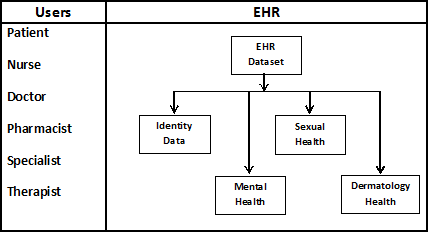
\includegraphics[width=15cm,height=8cm]{pic/taxonomyehr.png}
	\caption{Taxonomy of healthcare users}
	\label{fig:taxonomyehr}
\end{figure}

\item \textbf{Administration/Management of Health Organizations}\\
Health organizations should prepare a detailed study on security issues and address the protection of confidential patient data carefully. Because of the increasing challenges to health organizations, these organizations require another feature such as data management in addition to the privacy and security issues \cite{pr44}. Also, the network security in the healthcare systems requires the integration of all the different network units in the security system. In addition, the connection with \hlyellow{the proper adoption} of security context \hlyellow{of each device} in the network (such as a computer, sensor and phone). Furthermore, providing the vision of information with access control in real time helps to build a security efficient system for healthcare \cite{pr45}.

\end{itemize}

\subsection{To Propose a Model/Framework of Integrating WSN with Healthcare System}
In this section, we will explain the proposed model for the protection of patient information through the establishment of the healthcare scheme has security and efficiency. This proposal includes data protection in two areas of data collection (WSN) and server database (the Internet) as shown in Figure \ref{fig:poropsedmodel}. The components used in the proposed scheme are sensors nodes, communication devices (phone and iPad), a local and remote server. Sensor nodes used to gather patient information in an environment (hospital or clinic), communication devices used to send and receive medical information such as medical reports, these devices used by patients or medical staff and that are authorized access to confidential information. Servers \hlyellow{are used} to store patients' medical records and control access to a database. For example, a doctor in a hospital can send directives to the patients by sending a message to a nurse's device, and the latter sends this directive to patients through wireless networks. Also, the patient can obtain his medical record history via sending a message directly to the remote server over the Internet if the patient is authorized to grant access to his information. Collecting patient data through sensor nodes requires protection from the risks and threats \hlyellow{(such as internal and external attacks)}. Also, the transfer of patient's data from and to the server database online requires applying critical security policies \hlyellow{to prevent} the various attacks. Our framework offers the following capabilities to ensure the application of healthcare:
\begin{itemize}
\item Protection of WSN through encryption and signature \hlyellow{(ECC and ECDSA)}.
\item WSN data management and use of the proper context \hlyellow{(XML and XACML)} for the exchange of data on different devices.
\item Use of lightweight algorithms to address the performance and security.
\item Controlled access for authorized users and the database management via the Internet.
\end{itemize}

%fig4
\begin{figure}[t]
	\centering
		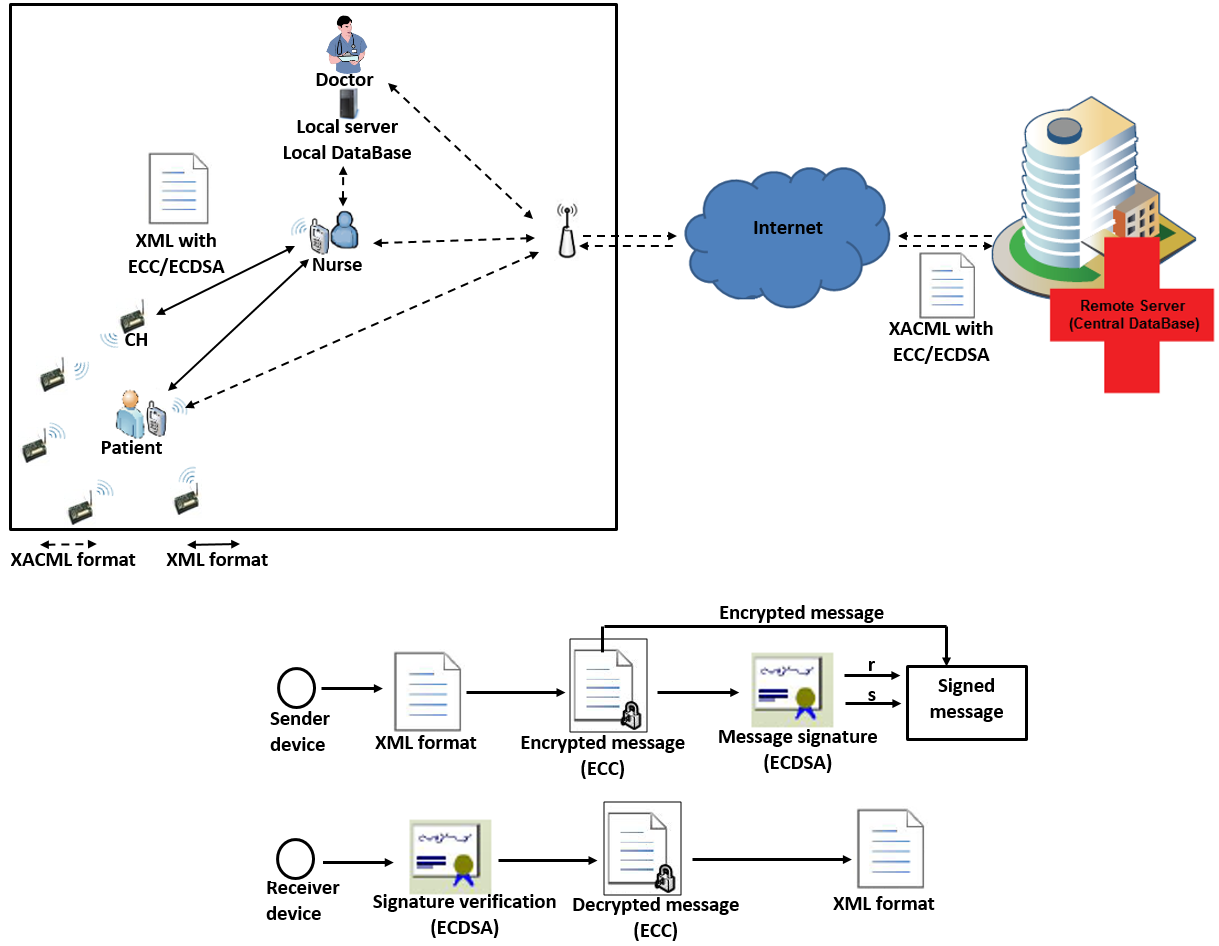
\includegraphics[width=15cm,height=13cm]{pic/poropsedmodel.png}
	\caption{The proposed model in hospital or clinic environment}
	\label{fig:poropsedmodel}
\end{figure}

\subsection{To Design Protocols to Improve the Security of WSN and EHR}
In this section, we propose a set of security mechanisms to use in healthcare application based on WSN.
\begin{enumerate}

\item \textbf{Quark Hash with ECDSA to Improve the Integrity and Authentication of EHR}\\
The hash algorithm is one of the important processes used by the ECDSA algorithm to complete the signing. ECDSA algorithm uses a secure hash algorithm (SHA-1) provided by NIST in 1995 to preserve the message integrity. This algorithm produces a digest 160-bit size with 6122 gate-equivalent (GE), where it needs the complex operations to accomplish digesting message. In digital signatures, the hash algorithm should be collisions \cite{pr29}, preimage and 2 preimage resistance \cite{pr32}. Authors in \cite{pr32,pr30,pr31,pr29} pointed out that this algorithm can suffer from collision and preimage. But SHA-1 is still used in many signature algorithms such as ECDSA. We propose using the Quark hash algorithm for signature in ECDSA rather than the SHA-1. Quark algorithm produces digest 136-bit size with 1379 GE. This algorithm was presented 2010 by authors in \cite{p7} in order to reduce the memory, energy requirements and resistance to attacks. Quark is faster and lighter than the SHA-1 algorithm. Also, this algorithm is resistant to attacks such as collisions, multicollision, distinguishers, preimage and 2nd preimage.

\item \textbf{Healthcare Data Management by XML to Improve the EHR's Storing/Exchanging}\\
Different systems that use a variety of devices require data management to be efficient. In our scheme, we use different devices such as sensors, phones and computers (servers). Therefore, we need a technology that allows for compatibility and data exchange among different devices. We propose the use of XML to manage the WLAN data. This descriptive language enables all devices to read data in a simple and meaningful way. In addition, we suggest using the mechanisms of encryption and signature (ECC/ECDSA) with XML file for the management and protection of patient data at the same time.

\item \textbf{Healthcare Security Using Signencryption to EHR Confidentiality}\\
ECDSA algorithm accomplishes operations \hlyellow{of the public key, signature generation} and signature verification. The operation of signature verification in ECDSA algorithm consumes more time and energy than a signature generation \cite{p11, p15}. We assume that we have a hospital care scheme as shown in Figure \ref{fig:hospitalcare}. We propose using homomorphic property with signencryption (the signature with encryption) in all sensor nodes. Homomorphic property means the direct computation on encrypted data. Each sensor node signs the message and then encrypts it, and sends it to the cluster head (CH). CH combines all signed and encrypted messages without decrypts or verifies the message. Afterward, CH sends encrypted messages to a nurse. The collection of encrypted messages without decrypt in the CH reduces the transport operations (where the transport operations consume more energy from the computation operations) and thus save time and energy.

%fig5
\begin{figure}[t]
	\centering
		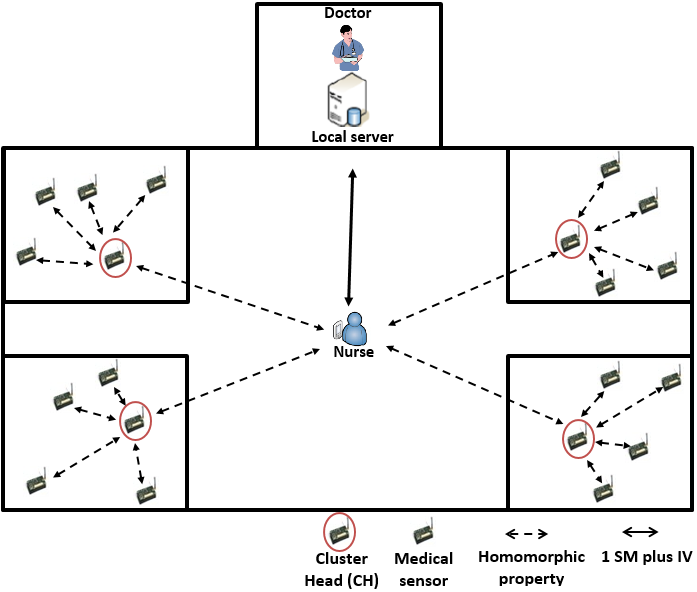
\includegraphics[width=13cm,height=10cm]{pic/hospitalcare.png}
	\caption{Homomorphic and 1 scalar multiplication with signencryption}
	\label{fig:hospitalcare}
\end{figure}

The second part of this scheme is to use 1 scalar multiplication (SM) in signature verification with the intermediate value (IV), where IV with a message encrypted signature is sent from the nurse device to the server (doctor device). IV includes 1 SM's result, ID, time and public key, and encrypts by SHA-1. Signature verification in ECDSA algorithm uses 2 SM. \hlyellow{The SM operation consumes more time and energy in the signature verification \cite{p17, p46}. This process will reduce the complexity of operations on the server device by calculating 1 SM + IV instead of the 2 SM}. Therefore, we suggest using homomorphic property with all sensor nodes and 1 SM (prime field) of nurse device to the server. The use of the prime field with this approach offers more security than binary field \cite{p26}. These processes lead to improved ECDSA performance to secure healthcare applications.

\item \textbf{Anonymity with ECDSA Privacy}\\
The ECDSA algorithm is used to perform the integrity of the messages. This algorithm prevents the attacker from changing the message data, since any change in the message will be discovered by the receiver. ECDSA produce the signing of the message ($r,s$) where r is the value used to calculate the signature in the process of signature verification and $s$ is the signature.
The sender signs the message ($m$) by ECDSA and gets ($r,s$). The sender sends the message $m$, $r$ and $s$ to the receiver, who checks the message. There are some of the attacks carried out on the $r$ and $s$ to get the private key $d$. If the attacker is able to get $d$, this attacker can produce the same original signatures. Side channel attack (SCA) can penetrate ECDSA signatures and thus get $d$ (Where $d$ is the security in this algorithm, if the attacker discovered the private key, data is easily penetrated). These attacks rely on information leaked to the ephemeral key ($k$) and the value of $r$ is available publicly. 

We propose adding anonymity property to ECDSA's signature to hide information of a signature's parameters $r$ and $s$ from the attackers through adding two unreal signatures ($r1,s1$) and ($r2,s2$). Moreover, we accomplish this property in the original signature ($r,s$) depending on the value of $k$. If the value of $k$ is odd, we divide each of $r$ and $s$ into three parts, while if the value of k is even, we divide each of $r$ and $s$ into four parts and exchange parts (where each of $r$ and $s$ have the same number of bits). After the completion of this operation, the value is sent with the message to specify the odd or even division in the receiver. Afterward, the receiver can verify that the message returns the same parts of the $r$ and $s$ to its original place. When using a key length of 384-bit in the case of the division of $r$ and $s$ bits into three parts (odd case), the length of each part is 128-bit. In the case of division into four parts (even case), the length of each part is 96-bit. When using a key length of 521-bit, we add padding 19-bit for a total of bits is 540-bit. Therefore, the length of each part in the odd case is a 180-bit while in the even case is 135-bit. In both odd and even cases to the value of $k$ is replacing two parts between $r$ and $s$. This mechanism prevents attacks from penetrating ECDSA signature because the attacker when he gets on the value of $r$ and $s$, he has not the original value for $r$ and $s$. Then, this attacker cannot derive the private key and thereby protect patient's data from the change.


\item \textbf{Access Control with EHR Database to Improve the Authorization of Healthcare Users}\\
The other important part of healthcare applications is to protect patient's data stored in the server database. These data need protection mechanisms of internal and external attackers. Therefore, patients' database in the server requires defining the access privileges of each user (nurse, doctor, pharmacist, practitioner) wants access to this data. The access control (AC) property only allows authorized users access to certain data. AC provides confidentiality in the EHR by restricting access rights for authorized users \cite{pr27}. 

We propose to merge two models role-based (RBAC) and attribute-based access control (ABAC) to specify the role of each user with a specific task and attributes that grant more privileges. We propose the use of features XACML and anonymity to protect patient's data from illegal and unauthorized access. Initially, users (employees or patients) should be authenticated to the HWSN application to prevent external attackers through the use of signencryption (ECC/ECDSA). The next stage is the use of XACML to determine the information that the user can access. At this stage, our application involves identifying the capabilities of each user (reading, writing), to identify access each user to certain data and define the tasks of each user. Suppose the patient's information is stored in the databases and only the hospital administrator has the authority to access all information. We propose to add an anonymity property with XACML by concealing some fields for some users. We assume the use of three databases (patients' identifications, the health information of the patients and professionals' identifications). Each patient has a number and pseudonym in the central database in addition to the use of the concept of multiple definitions of the various diseases for the one pseudonym. For example, if a patient is suffering from several diseases, there is definition for each disease, where the patient number, health institution number ($h_i$), the central pseudonym of the patient ($p_i$) with a pseudonym for each disease ($d_i$) are encrypted. This means that the patient's definition differs whether within the one health institution or many health institutions. In our scheme, we propose encryption of the properties and personal information in XACML file. XACML defines the policies and the semantic to apply those policies. XACML formats are used for request and response between the entities policy enforcement point (PEP) and policy decision point (PDP) to determine access control of the source \cite{pr42} (as shown in Figure \ref{fig:xacmlops}). Furthermore, XACML is composed of policies and rules. Policies define the applied of request, while the rules governing limitations for the applied of XACML. The request consists of attributes associated with the request sender and the response contains the decision (permit, deny, not applicable and indeterminate).

%fig6
\begin{figure}[t]
	\centering
		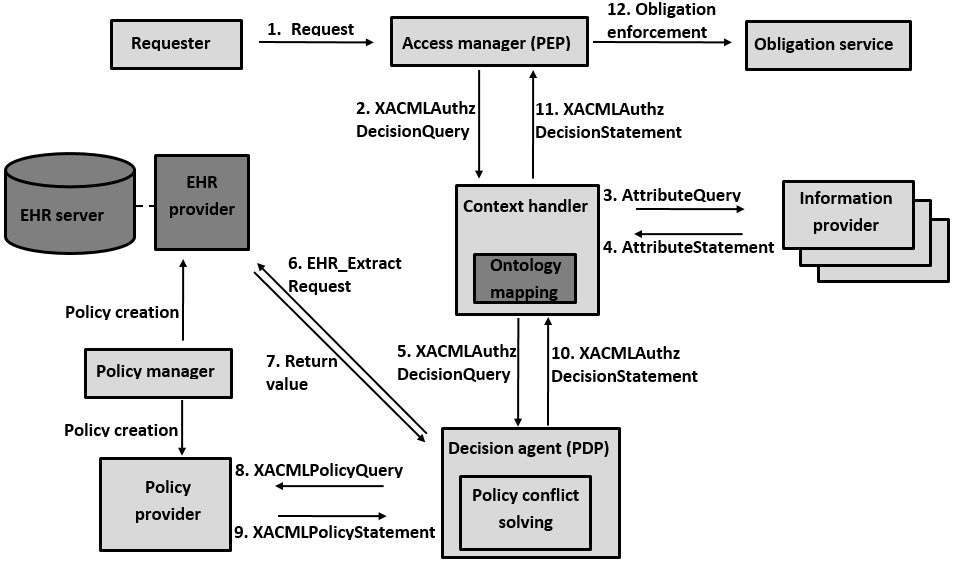
\includegraphics[width=18cm,height=12cm]{pic/xacmloperations.png}
	\caption{XACML operations \cite{pr48}}
	\label{fig:xacmlops}
\end{figure}

\textbf{Anonymity property} is applied to the patient data by concealing data about a user who is not required to know. For example, the nurse is not required to know the information about patient identification, but it is possible to know information such as the medical name (pseudonym), the range of age and medical reports. The doctor can know the personal information of the patient, but it is not important to know the criminal status of the patient information. In addition, if a doctor asked to consult another doctor, the latter is allowed to access only health information and medical reports. The addition of anonymity property with XACML leads to increase the privacy of data through the hide data and limit access for authorized users.
\end{enumerate}

\subsection{To Use Simulation Technique to Develop an Healthcare System}
In this section, we will explain application tools and algorithms implementation for our research objectives.
\begin{enumerate}

\item \textbf{Application Tools of the Study Objectives}\\
Theoretical objectives need tools to be applied. Firstly, we propose to simulate all of these objectives in a network simulator (NS3). This simulator has the ability to integrate the schemes in both simulation and real environments. It is a powerful tool to simulate types of different networks. It provides performance and memory management better than other simulators. This simulation supports many features such as C++ language, protocols closer for the real world, open source networking and virtualization. \hlyellow{The NS3 will be used to simulate/test the protocols only and not to simulate network attacks by hackers}. Secondly, we apply these objectives in the real world using a sensor mote. We can evaluate and compare the results simulation and the real world to validate the viability of executing these objectives in healthcare applications based WSN.

\item \textbf{Algorithms Implementation to Enhance Privacy of HWSN Application}\\
Sharing EHR among the healthcare professionals and the patient raises genuine security concerns. To minimize these concerns, we plan to anonymize the EHR's entries in the repository before disclosing it to the users. The k-anonymity is A popular method to anonymize patients' data. The use of k-anonymity \cite{pr22} an essential EHR's dataset can be sent safely, it is hidden and difficult for a malicious user to recognize the right identities for users in the EHR's repository. 
\end{enumerate}

\section{Expected Outcomes and Research Timelines}
Our ultimate goal is to improve the life quality of human society, in particular, patient healthcare plus maximizing the benefits of modern technology and the final product is an efficient but the secure healthcare system preserving patient's privacy. We focus on the expected results of our project's research on the following:
\begin{enumerate}
\item After doing a comprehensive survey on ECC \hlyellow{(our survey paper)} specified as \textbf{Task 1} in Section 3.2, we anticipate a journal publication on \emph{IEEE Security and Privacy}. In this article, we will evaluate the ECC algorithms such as ECDSA and ECDH, and obtain some \hlyellow{insight to implement} these algorithms in WSN.

\item All study efforts and activities in Section 3.3 can be summarized into 3 tasks:
     \begin{itemize}
           \item \textbf{Task 2.1}: to structure patient information.  
           \item \textbf{Task 2.2}: to classify healthcare users and healthcare providers.
           \item \textbf{Task 2.3}: to access control to the information.
     \end{itemize}
     \textbf{Task 2.1} and \textbf{Task 2.2} result is a user model and a service model such two models will provide us with a platform to closely look into the healthcare services characteristics and features. The findings of completing \textbf{Task 2.1} and \textbf{Task 2.2} will be included in a research paper, which might be published on a \emph{medical healthcare conference or journal}. It is expected from \textbf{Task 2.3} that a practical healthcare \hlyellow{web system} be developed. It is possible to consolidate the research paper and the implementation/experiment result in \textbf{Task 2.3} into a journal paper (\emph{International Journal of Medical Informatics}).
     
\item What is described in Section 3.4 can be \textbf{Task 3.1}. An EHR repository that incorporates WSN can assist in collecting real-time healthcare data such as repository rate, blood pressure and heart rate. Tasks to accomplish in Section 3.5 include:
\begin{itemize}
           \item \textbf{Task 3.2}: to design a service protocol for WSN to collect patients' physiological data without intruding on patients' personal life.  
           \item \textbf{Task 3.3}: to develop a communication protocol for WSN to transport healthcare data to the EHR repository.      
     \end{itemize}

\textbf{Task 3.2} involves allocating sensor nodes in the room or hospital bed where the patient would routinely reside. \textbf{Task 3.3} is about how the WSN communicates with the healthcare services. As soon as WSN collects some physiological data, either WSN sends a signal to the doctor if there is an emergency or transport them to the patient EHR repository, so the WSN must authenticate itself with a doctor or the server or which patients' EHR are stored. We would write a paper describing the strategies and protocols for our proposed WSN based healthcare application.

\item Based on the practical healthcare system and the model of WSN, we will accomplish the development of algorithms/protocols \hlyellow{using of simulation and real environment} which guarantee the security in \textbf{Task 4}. Section 3.5 in the methodology Section primarily addresses the security issues which might be involved in the proposed healthcare system. We divide all of these into 5 tasks.

  \begin{itemize}
           \item \textbf{Task 4.1}: to replace the SHA-1 hash algorithm in ECDSA algorithm with a Quark hash.
           \item \textbf{Task 4.2}: to structure healthcare data by taking advantage of XML technology.
           \item \textbf{Task 4.3}: to utilize signencryption in EHR storage in the repository.
           \item \textbf{Task 4.4}: to hide ECDSA parameters by use of anonymity property.
           \item \textbf{Task 4.5}: to develop a new authorisation/paradigm based on the XACML to access/manage the EHR repository.
     \end{itemize}
All the results or findings from \textbf{Task 4.1-4.5} will form the main body of the PhD thesis, which is all publishable in a \emph{high impact index journal}.

\item \textbf{Task 5}: a complete dissertation in fulfilment of requirement PhD degree. 
\end{enumerate}

Figure \ref{fig:timeline} represented by a Gantt chart, shows the time-line and expected results in our project search.




%fig7
\begin{figure}[ht]
	\centering
		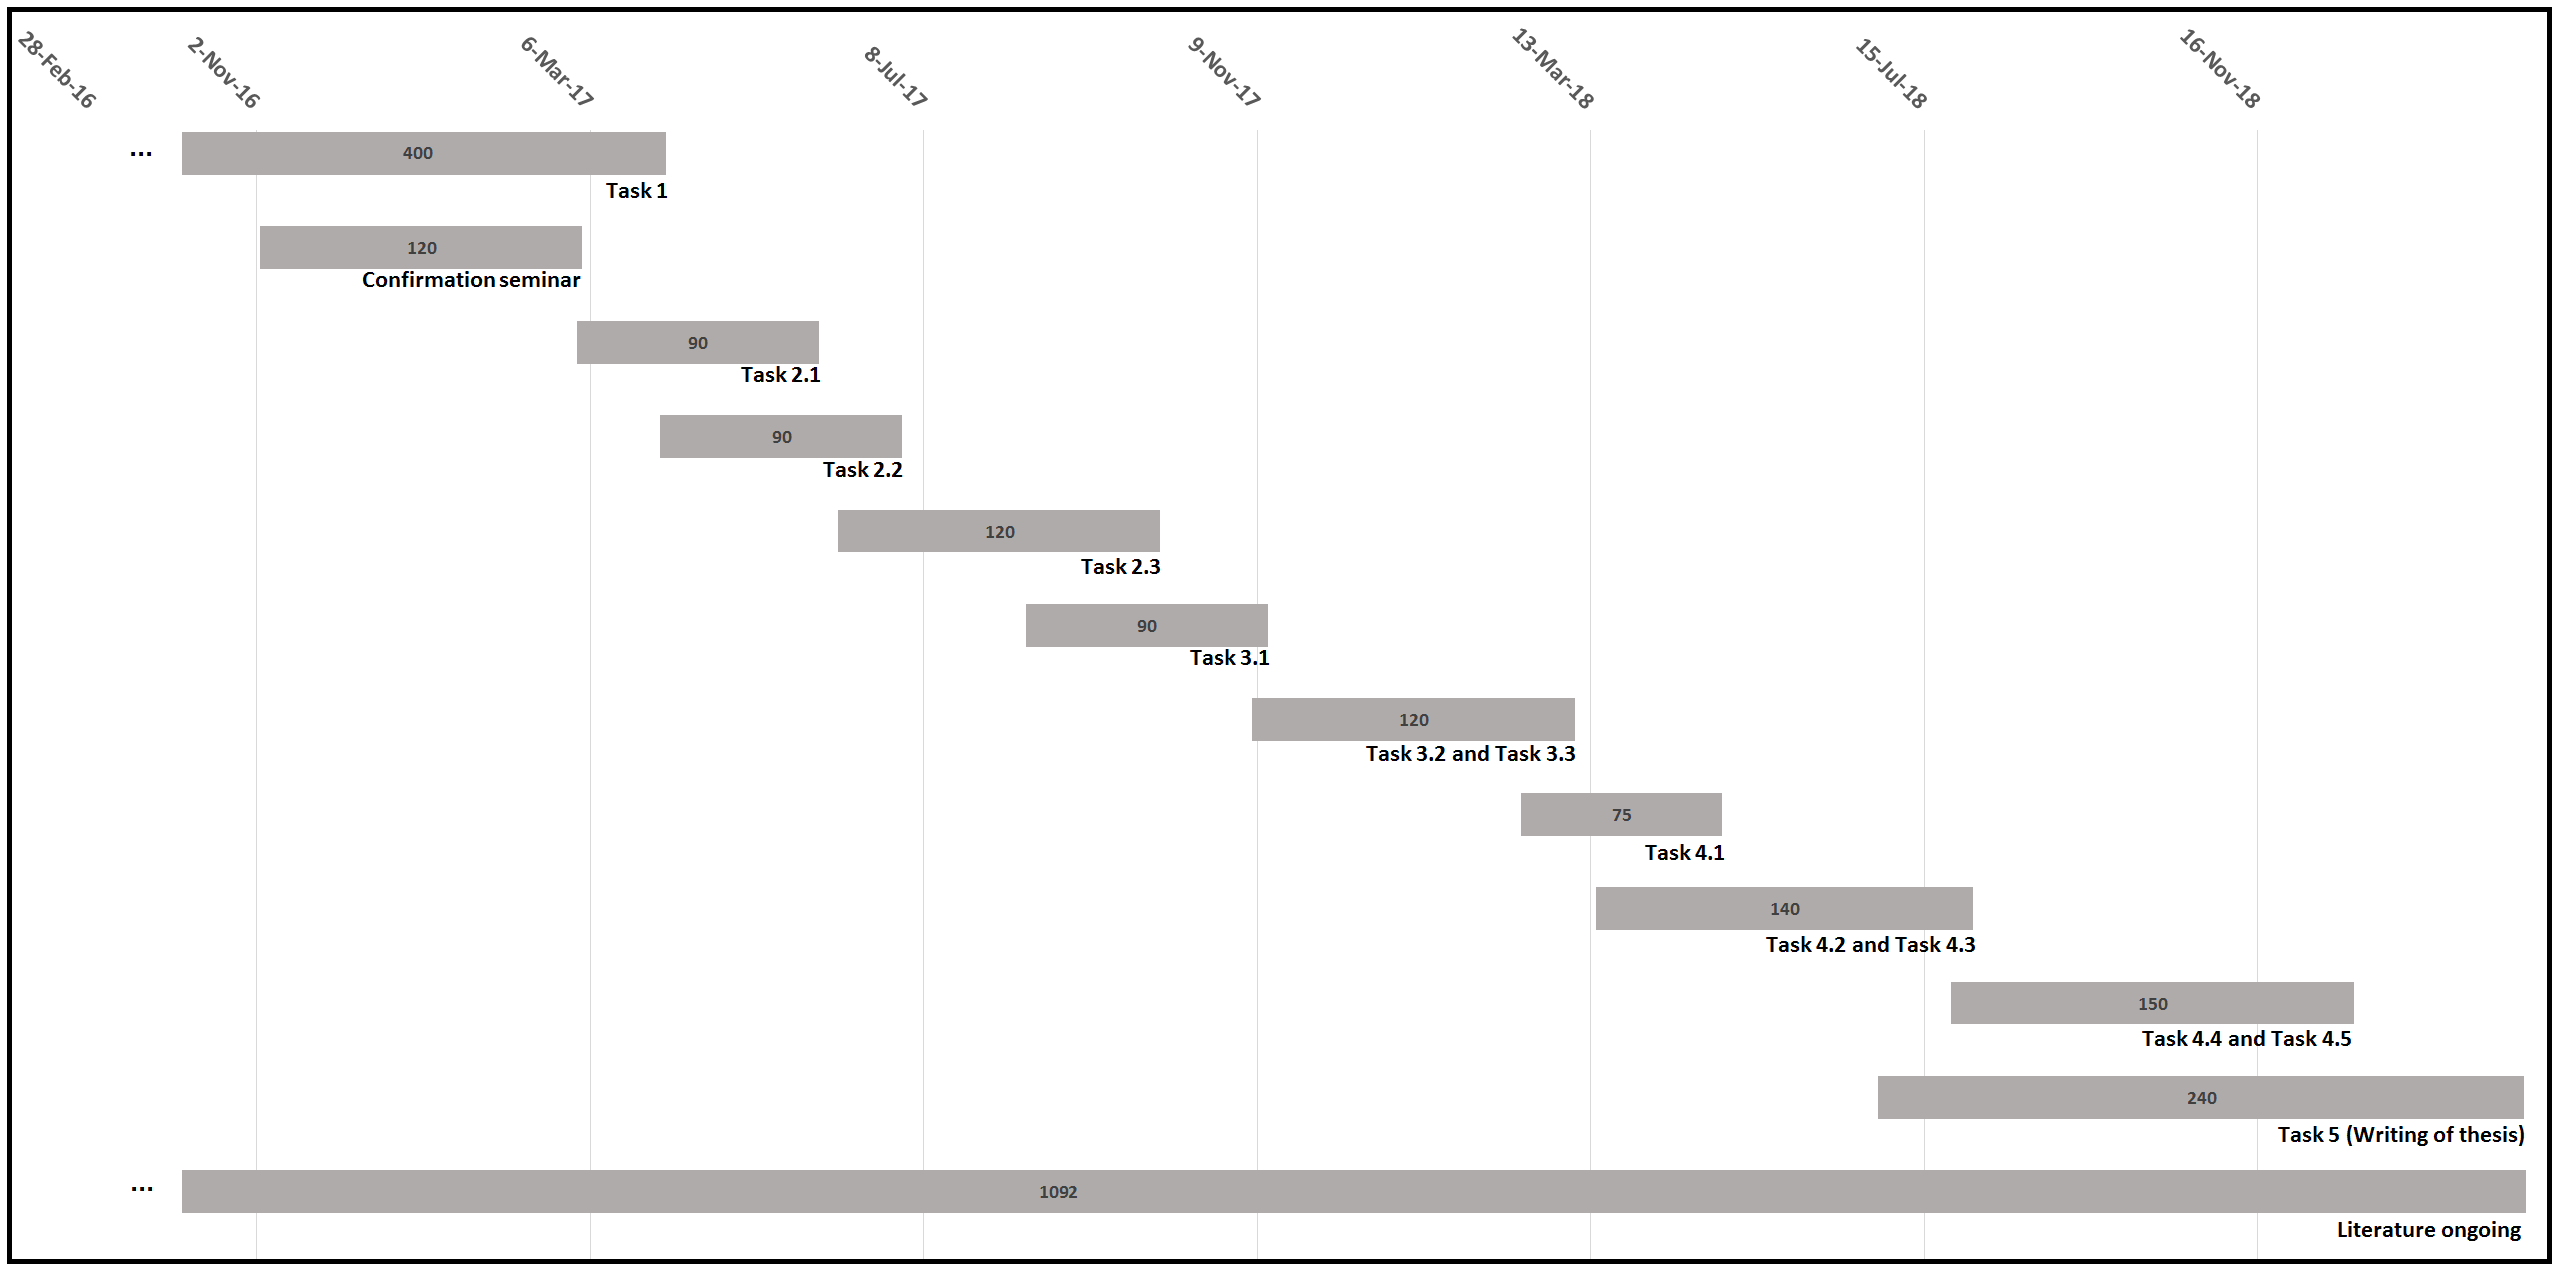
\includegraphics[angle=90,width=17cm,height=25cm]{pic/timeline.png}
	\caption{The proposed research time-line}
	\label{fig:timeline}
\end{figure}

\section{Preliminary Results}
Up to now, we have investigated security in healthcare applications based WSN and found that these applications needed quick and secure algorithms to protect patients' data from intruders. During our study, we found that the best encryption algorithms that provide fast computations, high-level of security, small keys and key distribution are ECC/ECDSA algorithms. When we investigated ECC/ECDSA algorithms and we found them suffering from some problems (such as complexity operations of the hash algorithm and SM, and leaked information) and needed some security and performance requirements for application in healthcare based WSN. Therefore, the preliminary results of our research are as the following.

\begin{itemize}
\item Survey paper for ECC/ECDSA algorithms.\\
\hlyellow{We have investigated asymmetric cryptographic algorithms during our survey paper. We found that ECC/ECDSA is the best algorithm to be used with source-restricted devices in terms of security and efficiency. This step is very important in our research project of building a healthcare application based on WSN}.

\item Implementation of mobile ad hoc network (MANET) in NS3 (C++).\\
\hlyellow{Our research project is a MANET network consisting of sensors and computers. We implemented MANET in NS3 as a primitive scheme to implement our proposed protocols/algorithms}.

\item Implementation of Quark algorithm in NS3.\\
\hlyellow{We implemented the Quark algorithm to integrate with ECDSA. After completing this protocol in our research project we will test the results of both ECDSA with SHA-1 and ECDSA with Quark on the level of security and efficiency}.

\item Implementation ECDSA in C++ language.\\
\hlyellow{We implemented the ECDSA algorithm in C ++ and will implement it in NS3 to assess security level, energy consumption, data size, delay and time when signing and verifying patient data as the basic algorithm in our scheme}.

\item Get free patients' data for the use of the public in the websites \textbf{Dartmouth Atlas of Health Care and phpartners}, and that benefits us in the operations of gathering information in \hlyellow{WSN when we will use NS3}.\\
\url{http://www.dartmouthatlas.org/}\\
\url{http://phpartners.org/health_stats.html#National%20Public%20Health%20Data%20Sets}

\end{itemize}


\clearpage
%\newpage
\onehalfspacing
%\singlespacing
\bibliographystyle{plainnat}
\bibliography{proposal}

\end{document}